        \subsection{correlation}

\begin{frame}{signal similarity}{correlation function}
	correlation function: compute similarity between two \textbf{stationary} signals $x$,$y$
    \begin{equation}
        r_\mathrm{xy}(\tau)=\mathcal{E}\lbrace x(t)y(t+\tau)\rbrace  
    \end{equation}  
	\pause
    
	\begin{itemize}
		\item	\textbf{continuous}:
            \begin{equation}
                r_\mathrm{xy}(\tau) = \int\limits_{-\infty}^{\infty}{x(t)\cdot y(t+\tau)dt}
            \end{equation}
		\item	\textbf{discrete}:
            \begin{equation}
                r_\mathrm{xy}(\eta) = \sum\limits_{i=-\infty}^{\infty}{x(i)\cdot y(i+\eta)}
            \end{equation}
	\end{itemize}
\end{frame}

\begin{frame}{signal similarity}{correlation function: animation}
    \vspace{-5mm}
    \begin{footnotesize}
    \begin{equation}
        r_\mathrm{xy}(\tau) = \int\limits_{-\infty}^{\infty}{x(t)\cdot y(t+\tau)}dt
    \end{equation}
    \end{footnotesize}
    \includevideo{video/XCorrAnimation.mp4}
\end{frame}

\begin{frame}{signal similarity}{correlation function: use cases}
    \begin{itemize}
        \item   find (linear!) similarity between two signals (e.g., clean and noisy)
        \item   find time shift between to similar signals
        \pause
        \bigskip
        \item   example: \textbf{radar}
            \begin{itemize}
                \item   correlate sent signal with received signal
                \item   pick maximum location and convert to distance of object
            \end{itemize}
    \end{itemize}
\end{frame}

\begin{frame}{signal similarity}{correlation coefficient}
    \begin{equation}\nonumber
        r_\mathrm{xy}(0) = \frac{\mathcal{E}\lbrace(X-\mu_X)(Y-\mu_Y)\rbrace}{\sigma_X\sigma_Y}
    \end{equation}
\end{frame}

\begin{frame}{signal similarity}{correlation function: problems as summary statistic}
Anscombe's quartet:
    \begin{itemize}
        \item   mean: 7.5, variance: 4.2
        \item   \textbf{Pearson correlation coefficient}: 0.816
    \end{itemize}
    \begin{figure}
        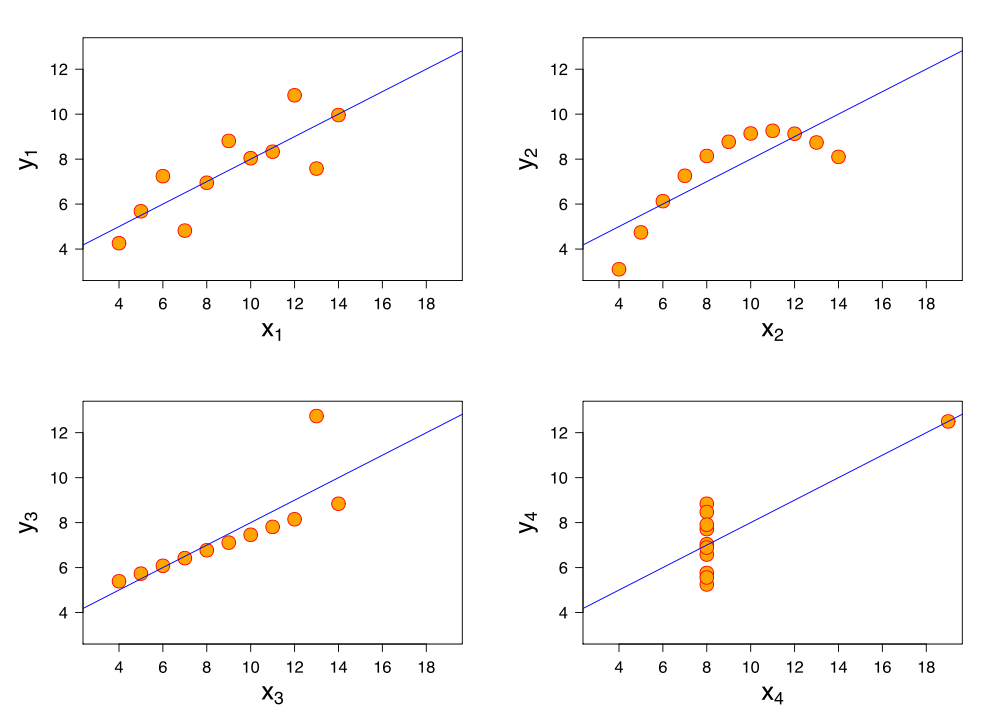
\includegraphics[scale=.2]{graph/Anscombes_quartet}
    \end{figure}
\end{frame}

\begin{frame}\frametitle{correlation function}\framesubtitle{correlation function: examples}
	\only<1>
	{
		\vspace{-15mm}
		\begin{columns}
			\column{5cm}
			Describe the (cross) correlation function between the following signals:
			
			\column{4cm}
			%\hspace{5mm}
			\begin{flushright}
				 
\includegraphics[scale=.08]{Graph/question-mark}
			\end{flushright}
		\end{columns}
	
		\begin{itemize}
			\item	rectangular window vs.
			\item	sine vs.
			\item	noise
		\end{itemize}
	}

	\only<2>
	{
		\vspace{-5mm}
		\begin{figure}
			\centering
				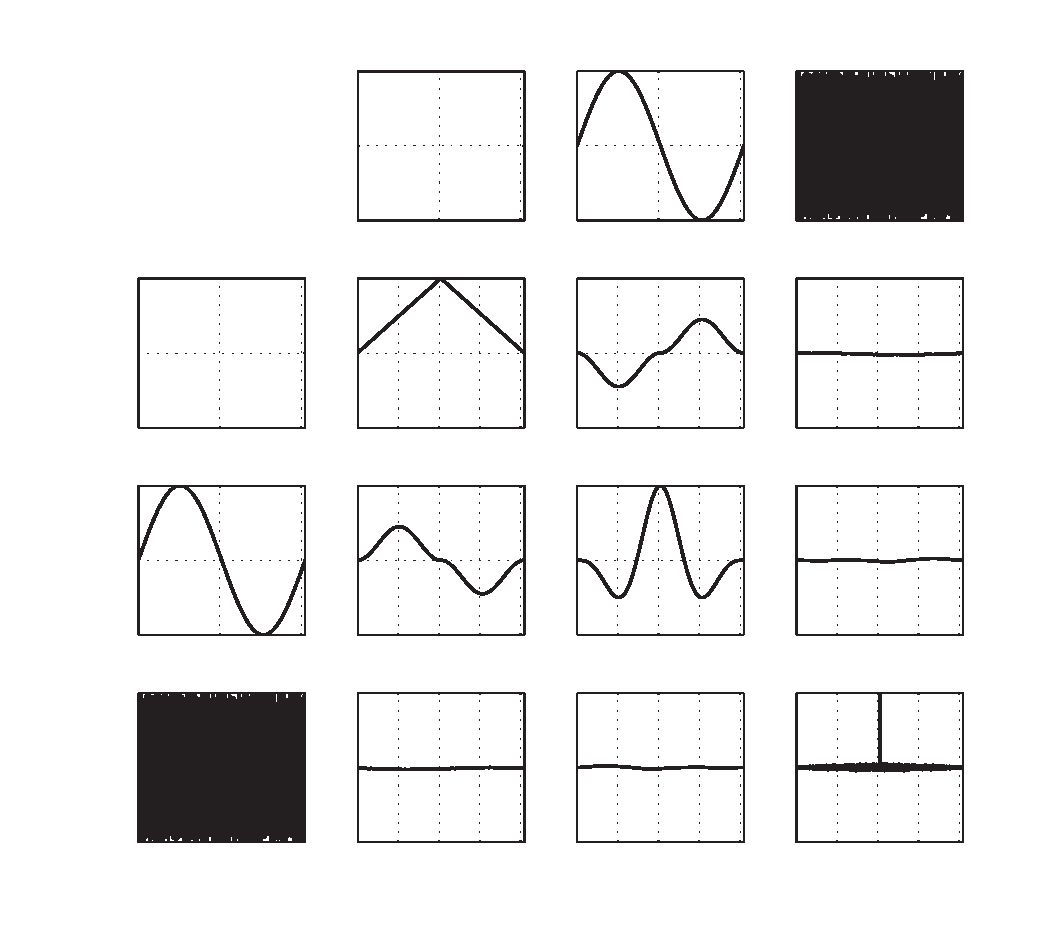
\includegraphics[scale=.5]{graph/xcorr}
			\label{fig:xcorr}
		\end{figure}
	}
	%\only<3>
	%{
        %HAVE A VIDEO HERE!
		%%\begin{figure}
			%%\includemovie[poster,mouse=true]{\linewidth}{.6\linewidth}{video/animatecorr.avi}
		%%\end{figure}
	%}
\end{frame}

\begin{frame}\frametitle{correlation function}\framesubtitle{correlation function: examples}
    \includevideo{video/XCorrAnimation2.mp4}
\end{frame}	

\begin{frame}{correlation function}{auto correlation function}
		\begin{equation}
			r_\mathrm{xx}(\tau)=\mathcal{E}\lbrace x(t)x(t+\tau)\rbrace  
		\end{equation}

		\pause
		\begin{block}{autocorrelation function properties}
			\begin{itemize}
				\item	\textbf{power}: $r_{xx}(0) = 	\mathcal{E}\lbrace X^2\rbrace $ 

				\pause
				\item	\textbf{symmetry} $r_{xx}(\tau)=r_{xx}(-\tau)$\\
					(substitute $t=t'+\tau$)

				\pause
				\item	\textbf{global max}: $r_{xx}(\tau)\leq r_{xx}(0)$ 
					%(Binomial theorem $E\left\lbrace \big(x(t)x(t-\tau)\big)^2\right\rbrace $ )

				\pause
				\item	\textbf{periodicity}:\\
					The {ACF} of a periodic signal is periodic (period length of input signal)

			\end{itemize}	
		\end{block}
\end{frame}	

%\begin{frame}{correlation and power spectral density}{PSD}
	%\begin{itemize}
		%\item	\textbf{problem}: how to calculate the spectrum of a random process?
				%\begin{itemize}
					%\item	no analytic function to integrate
				%\end{itemize}
				%
		%\pause
		%\item	\textbf{solution}: Wiener-Khinchin theorem
		%\pause
		%\begin{equation}
			%S_{xx}(\omega) = \mathfrak{F}\lbrace \varphi_{xx}(\tau)\rbrace 
		%\end{equation}
	%\end{itemize}
%\end{frame}
%
%\begin{frame}{correlation and power spectral density}{PSD: properties}
%
		%\begin{block}{PSD properties}
			%\begin{itemize}
				%\item	\textbf{real} (symmetry in time domain!) 
%
				%\pause
				%\item	\textbf{power preservation}
					%\begin{equation}
						%\mathcal{E}\lbrace x^2\rbrace  = \varphi_{xx}(\tau = 0) = \frac{1}{2\pi}\int\limits_{-\infty}^{\infty}{S_{xx}(\omega)\enspace d\omega} 
					%\end{equation}
			%\end{itemize}	
		%\end{block}
%\end{frame}	
%
%\begin{frame}{correlation and power spectral density}{PSD: discrete signals}
	%\begin{itemize}
		%\item	\textbf{correlation}
				%\begin{equation}
					%\varphi_{xx}(l) = \mathcal{E}\lbrace x(n)\cdot x(n-l)\rbrace 
				%\end{equation}
		%\pause
		%\item	\textbf{PSD}
				%\begin{equation}
					%\varphi_{xx}(l) = \mathfrak{F^{-1}}\lbrace S_{xx}(\Omega)\rbrace =\frac{1}{2\pi}\int\limits_{-\pi}^{+\pi}S_{xx}(\Omega)e^{j\Omega l}\enspace d\Omega
				%\end{equation}  
		%\pause
		%\item	\textbf{power}
				%\begin{equation}
					%\varphi_{xx}(0)=\frac{1}{2\pi}\int\limits_{-\pi}^{+\pi}S_{xx}(\Omega)\enspace d\Omega
				%\end{equation}
	%\end{itemize}
%\end{frame}	
